\documentclass[svgnames,11pt]{beamer}
\input{/home/tof/Documents/Cozy/latex-include/preambule_commun.tex}
\input{/home/tof/Documents/Cozy/latex-include/preambule_beamer.tex}
\usepackage{pgfpages} \setbeameroption{show notes on second screen=left}
\author[]{Christophe Viroulaud}
\title{Programmation assembleur}
\date{}
%\logo{}
\institute{Première - NSI}

\begin{document}
\begin{frame}
    \titlepage
\end{frame}
\begin{frame}
    \frametitle{}

    L'\emph{unité de contrôle} d'un processeur lit des instructions contenues dans la mémoire et ordonne à l'\emph{unité arithmétique et logique} de les exécuter. Cependant, le processeur ne comprend pas le langage humain et des consignes même simples ne sont pas directement interprétables par la machine.

\end{frame}
\begin{frame}
    \frametitle{}

    \begin{center}
        \framebox{Comment l'Homme communique avec la machine?}
    \end{center}

\end{frame}
\section{Langage machine}
\subsection{Langage binaire}
\begin{frame}
    \frametitle{Langage machine}

    \begin{aretenir}[]
        Un processeur est un composant électronique: il n'interprète que des signaux électriques.
    \end{aretenir}

\end{frame}
\begin{frame}
    \frametitle{}

    Techniquement il ne peut y avoir que deux états:
    \begin{itemize}
        \item passage de courant électrique représenté par le chiffre 1,
        \item absence de courant électrique représenté par le chiffre 0.
    \end{itemize}
    \begin{center}
        On parle de \textbf{langage binaire}.
    \end{center}
\end{frame}
\begin{frame}
    \frametitle{Un concept déjà existant}
    \begin{center}
        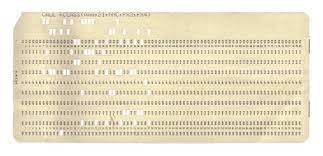
\includegraphics[width=4cm]{ressources/carte.jpg}

    \end{center}
    \begin{center}
        \centering
        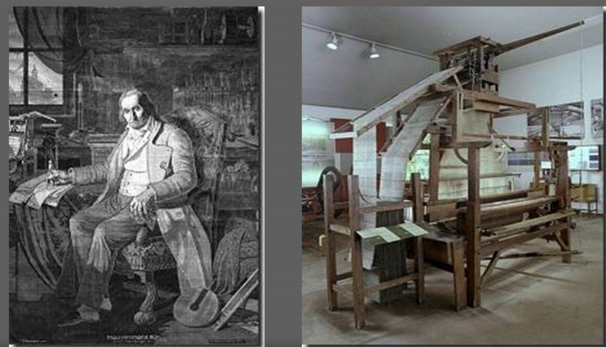
\includegraphics[width=6cm]{ressources/jacquard.png}
    \end{center}
    \begin{aretenir}[1801]
        Joseph-Marie Jacquard a développé un métier à tisser avec lequel le motif à tisser était déterminé par des cartes perforées.
    \end{aretenir}
\end{frame}
\begin{frame}
    \frametitle{Une théorie mathématique}
    \begin{center}
        \centering
        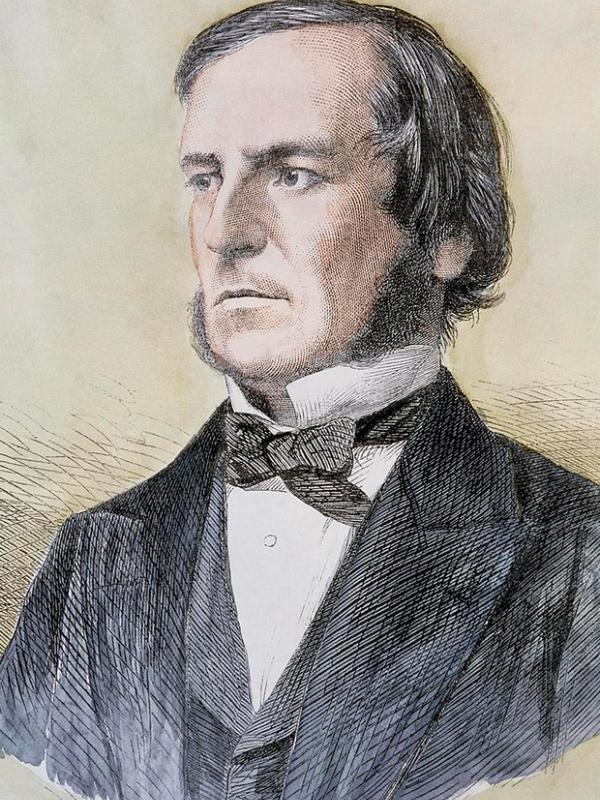
\includegraphics[width=4cm]{ressources/boole.jpg}
    \end{center}
    \begin{aretenir}[1844-1854]
        George Boole crée une algèbre binaire, dite booléenne, n'acceptant que deux valeurs numériques : 0 et 1.
    \end{aretenir}
    \note[item]{de nombreuses applications en électronique et informatique grâce à Claude Shannon dès 1938.}
    \note[item]{plus de détails dans un cours prochain.}
\end{frame}
\subsection{Langage de bas niveau}
\begin{frame}
    \frametitle{Langage de bas niveau}

    \begin{center}
        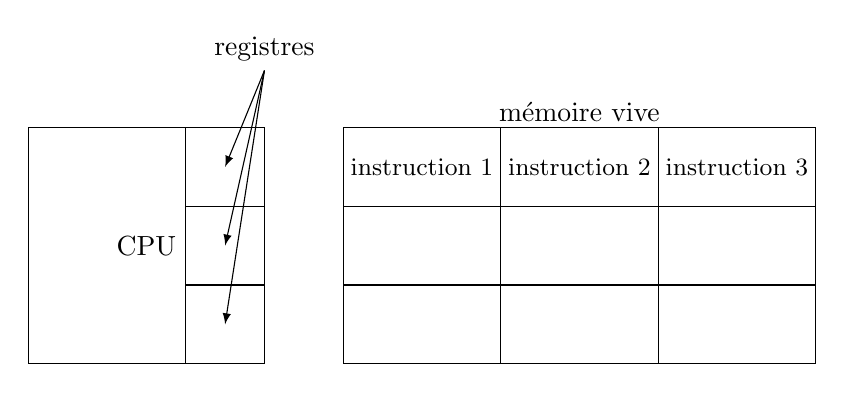
\begin{tikzpicture}
            \node[draw,minimum width=3cm,minimum height=3cm] (cpu) at (1.5,1.5){CPU};
            \draw (2,0) grid (3,3);
            \node at (7,3.2){mémoire vive};
            \draw (4,0) grid[xstep=2cm] (10,3);
            \node (registres) at (3,4){registres};
            \node at (5,2.5) {{\small instruction 1}};
            \node at (7,2.5) {{\small instruction 2}};
            \node at (9,2.5) {{\small instruction 3}};

            \draw[->,>=latex] (registres.south) -- (2.5,2.5);
            \draw[->,>=latex] (registres.south) -- (2.5,1.5);
            \draw[->,>=latex] (registres.south) -- (2.5,0.5);
        \end{tikzpicture}
        \captionof{figure}{Rappel: modèle de von Neumann}
    \end{center}
    \note[item]{registres = emplacement mémoire très rapide et très proche processeur (soudés à côté)}
    \note[item]{CPU = UA + UC}
    \note[item]{cpu va cherche instruction 1 puis 2\dots}
\end{frame}
\begin{frame}
    \frametitle{}

    Un processeur ne peut exécuter que des instructions basiques:
    \begin{itemize}
        \item<1-> \textbf{opérations arithmétiques:} \emph{\guill{additionne la valeur contenue dans le registre R1 et le nombre 789 et range le résultat dans le registre R0}}
        \item<2-> \textbf{transfert de données entre les registres et la mémoire vive:} \emph{\guill{prendre la valeur située à l’adresse mémoire 487 et la placer dans la registre R2}}
        \item<3-> \textbf{rupture de séquence:} \emph{\guill{saute de l'instruction 2 à l'instruction 5}}
    \end{itemize}

\end{frame}
\section{Langage assembleur}
\subsection{Un langage intermédiaire}
\begin{frame}
    \frametitle{Un langage intermédiaire}

    Le code \emph{0010 0110} donne l'ordre au processeur d'effectuer une multiplication.

\end{frame}
\begin{frame}
    \frametitle{}

    \begin{aretenir}[]
        Pour faciliter la vie des informaticiens, on remplace les code binaires par des \textbf{symboles mnémoniques}.

        \centering ADD, MOV, SUB\dots
    \end{aretenir}

\end{frame}
\subsection{Découverte d'un simulateur}

\begin{frame}[fragile]
    \frametitle{Découverte d'un simulateur}

    \begin{activite}
        \begin{enumerate}
            \item Ouvrir la page \url{https://www.peterhigginson.co.uk/ARMlite/}
            \item Repérer les éléments du modèle de von Neumann.
        \end{enumerate}
    \end{activite}
    \note{\fcolorbox{black}{red}{{\LARGE en mode TP à partir d'ici}}}
\end{frame}
\begin{frame}
    \frametitle{Correction}

    \begin{center}
        \centering
        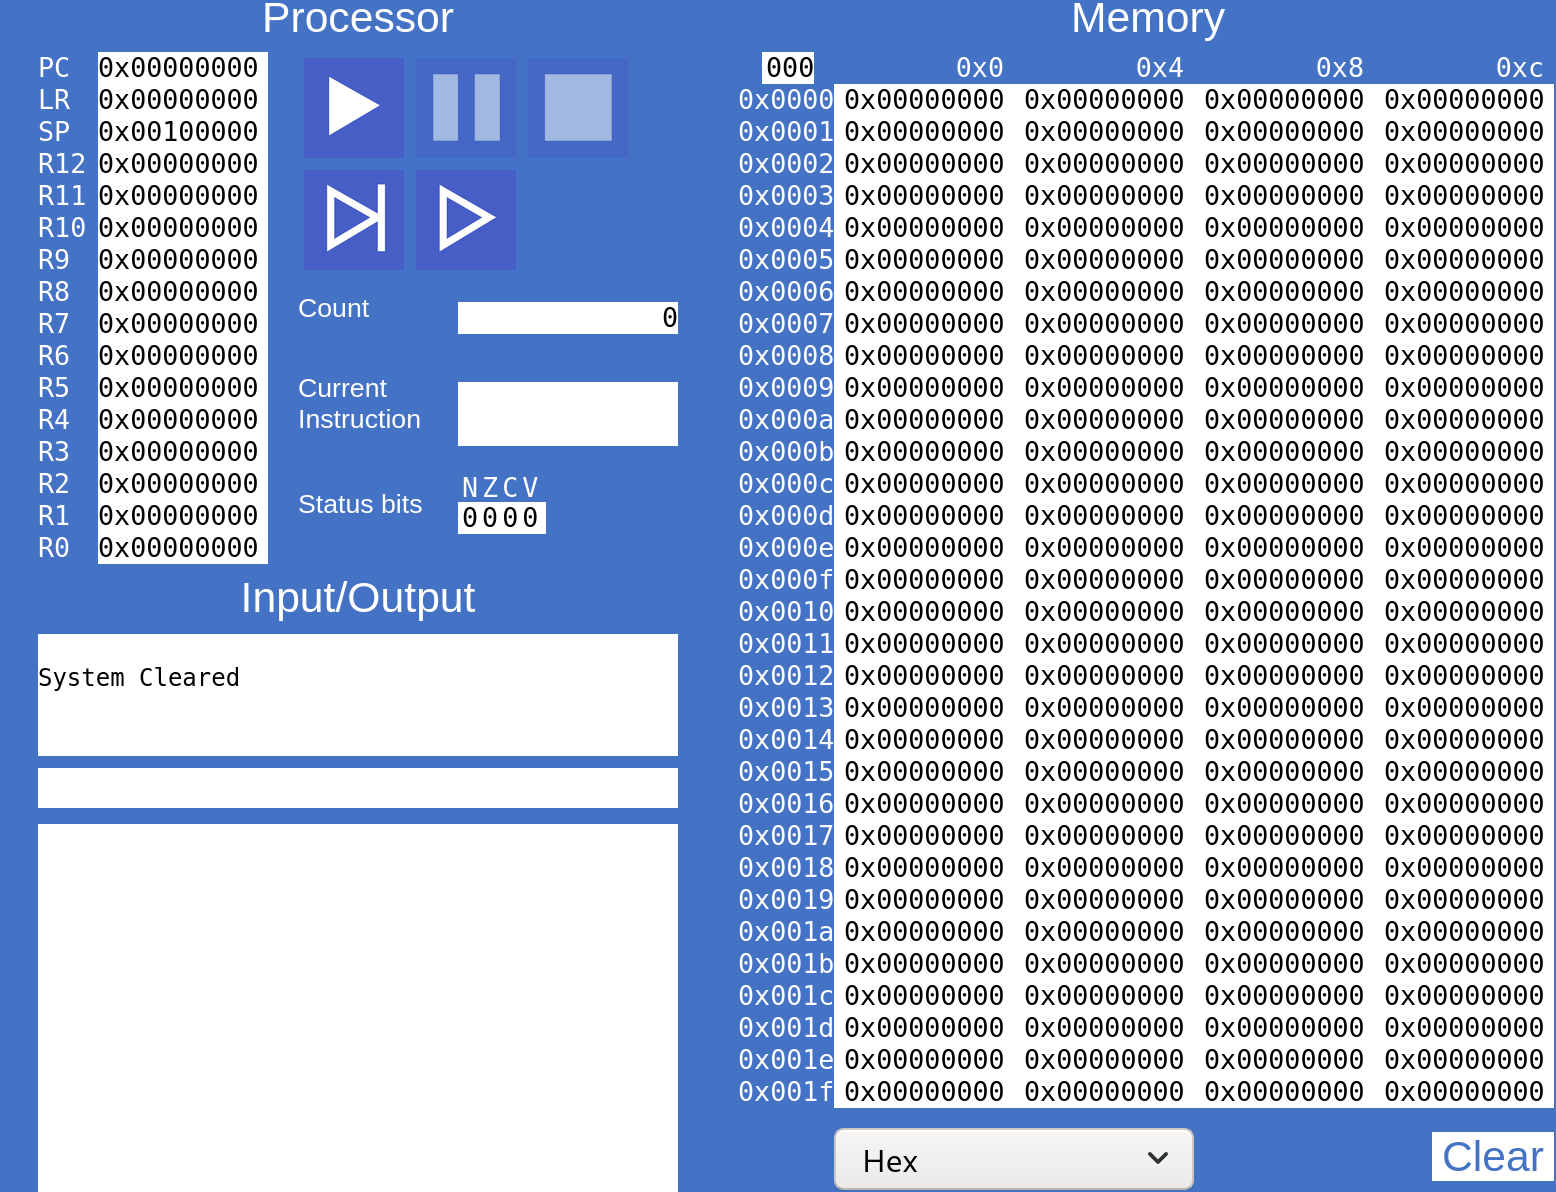
\includegraphics[width=9cm]{ressources/simulateur.png}
        \captionof{figure}{Simulateur 32-bit ARM}
        \label{IMG}
    \end{center}

\end{frame}
\begin{frame}[fragile]
    \frametitle{}

    \begin{activite}
        \begin{enumerate}
            \item Dans la partie \emph{Program} cliquer sur \emph{Edit} puis écrire les instructions suivantes:
                  \begin{center}
                      \begin{lstlisting}[language=Bash , basicstyle=\small, xleftmargin=2em, xrightmargin=2em]
MOV R0, #3
ADD R1,R0,#5
HALT
\end{lstlisting}
                  \end{center}
            \item Cliquer sur \emph{Submit} et observer ce qui se passe en mémoire.
            \item Cliquer sur le bouton \ref{pas} pour exécuter le programme.
                  \begin{center}
                      \centering
                      
\includegraphics[width=1cm]{ressources/pasapas.png}
                      \label{pas}
                      \captionof{figure}{Exécution pas à pas}
                  \end{center}
        \end{enumerate}
    \end{activite}

\end{frame}
\begin{frame}
    \frametitle{Correction}

    \begin{itemize}
        \item Le processeur exécute les instructions les unes après les autres.
        \item Les \textbf{mots-mémoires} sont présentés en \emph{hexadécimal}.
    \end{itemize}
    \begin{aretenir}[Commentaire]
        Dans cette première approche, nous afficherons les mots-mémoires et les données en

        \centering \textbf{Decimal (signed)}
    \end{aretenir}
    \note[item]{si pas halt, continue à lire les mot-mémoires.}
    \note[item]{passer en binaire aussi pour voir}
\end{frame}
\subsection{Opérations arithmétiques}
\begin{frame}
    \frametitle{Opérations arithmétiques}

    \begin{aretenir}[]
        Un processeur ne peut effectuer des calculs qu'avec des valeurs situées dans ses registres.
    \end{aretenir}

\end{frame}
\begin{frame}[fragile]
    \frametitle{}

    \begin{center}
        \begin{lstlisting}[language=C , basicstyle=\small, xleftmargin=2em, xrightmargin=2em]
ADD R0,R1,R2
\end{lstlisting}
        \captionof{code}{Ajoute la valeur du registre R2 à celle de R1 puis place le résultat dans R0.}
        \label{CODE}
    \end{center}
    \begin{center}
        \begin{lstlisting}[language=C , basicstyle=\small, xleftmargin=2em, xrightmargin=2em]
ADD R1,R1,#10
\end{lstlisting}
        \captionof{code}{Ajoute l'entier 10 à celle du registre R1 puis place le résultat dans R1.}
        \label{CODE}
    \end{center}
    Le symbole \emph{SUB} effectue une soustraction avec la même syntaxe.
\end{frame}
\begin{frame}
    \frametitle{Le compte est bon}

    \begin{activite}
        Dans le jeu du \emph{compte est bon} il faut retrouver un résultat à partir d'une série d'entiers. Dans cet exemple nous n'utiliserons que des additions et des soustractions.\\ La série de nombre est: 12 20 57 3
        \\
        Écrire un programme qui retrouve le résultat 52.
    \end{activite}

\end{frame}
\begin{frame}
    \frametitle{Avant de regarder la correction}
\begin{center}
    \centering
    \includegraphics[width=3cm]{/home/tof/Documents/Cozy/latex-include/stop.png}
    \end{center}
{\Large
    \begin{itemize}
        \item Prendre le temps de réfléchir,
        \item Analyser les messages d'erreur,
        \item Demander au professeur.
    \end{itemize}
}
\end{frame}
\begin{frame}[fragile]
    \frametitle{Correction}

    \begin{center}
        \begin{lstlisting}[language=C , basicstyle=\small, xleftmargin=2em, xrightmargin=2em]
ADD R0,R0,#57
ADD R0,R0,#3
ADD R0,R0,#12
SUB R0,R0,#20
HALT
\end{lstlisting}
        \captionof{code}{Un code possible}
        \label{CODE}
    \end{center}

\end{frame}
\subsection{Transfert de données}
\begin{frame}[fragile]
    \frametitle{Transfert de données}
Il est possible d'envoyer une valeur directement dans un registre.
\begin{center}
\begin{lstlisting}[language=C , basicstyle=\small, xleftmargin=2em, xrightmargin=2em]
MOV R0, #10
\end{lstlisting}
\captionof{code}{Place la valeur 10 dans R0.}
\label{CODE}
\end{center}
    

\end{frame}
\begin{frame}[fragile]
    \frametitle{}

    Il arrive régulièrement que les données soient déjà stockées dans la mémoire vive. Avant d'effectuer une opération arithmétique avec ces valeurs, il faut d'abord les charger dans les registres.
    \begin{center}
        \begin{lstlisting}[language=C , basicstyle=\small, xleftmargin=2em, xrightmargin=2em]
LDR R0,16
\end{lstlisting}
        \captionof{code}{\textbf{L}oa\textbf{DR}egister: charge dans R0 la valeur située à \textbf{l'adresse} 16 de la mémoire.}
        \label{CODE}
    \end{center}
\end{frame}
\begin{frame}[fragile]
    \frametitle{}

    \begin{center}
        \begin{lstlisting}[language=C , basicstyle=\small, xleftmargin=2em, xrightmargin=2em]
STR R0,20
\end{lstlisting}
        \captionof{code}{\textbf{ST}ore\textbf{R}egister: stocke la valeur de R0 dans l'espace mémoire situé à \textbf{l'adresse} 20.}
        \label{CODE}
    \end{center}

\end{frame}
\begin{frame}[fragile]
    \frametitle{}
Il semble fastidieux de demander au programmeur de manipuler les adresses mémoires. Heureusement il est possible d'assigner un \textbf{label} à un mot-mémoire.
    \begin{center}
        \begin{lstlisting}[language=C , basicstyle=\small, xleftmargin=2em, xrightmargin=2em]
LDR R0, mavaleur
HALT
mavaleur: 10
\end{lstlisting}
        \captionof{code}{charge dans R0 la valeur située dans la case mémoire \emph{mavaleur}.}
        \label{CODE}
        \end{center}

\end{frame}
\begin{frame}
    \frametitle{}

    \begin{activite}
    \begin{enumerate}
        \item Tester le programme précédent. Observer la valeur stockée en mémoire.
        \item Écrire un programme qui:
        \begin{itemize}
            \item stocke dans la mémoire vive les coordonnées \emph{x = 5} et \emph{y = 4} d'un personnage dans un jeu.
            \item modifie chaque coordonnée de 3 unités.
        \end{itemize}
    \end{enumerate}
    \end{activite}

\end{frame}
\begin{frame}
    \frametitle{Avant de regarder la correction}
\begin{center}
    \centering
    \includegraphics[width=3cm]{/home/tof/Documents/Cozy/latex-include/stop.png}
    \end{center}
{\Large
    \begin{itemize}
        \item Prendre le temps de réfléchir,
        \item Analyser les messages d'erreur,
        \item Demander au professeur.
    \end{itemize}
}
\end{frame}
\begin{frame}[fragile]
    \frametitle{Correction}

    \begin{center}
        \begin{lstlisting}[language=C , basicstyle=\small, xleftmargin=2em, xrightmargin=2em]
LDR R0, x
ADD R0, R0, #3
STR R0, x
LDR R1, y
ADD R1, R1, #3
STR R1, y
HALT
x: 5
y: 4
\end{lstlisting}
        \end{center}   

\end{frame}
\subsection{Rupture de séquence}
\begin{frame}[fragile]
    \frametitle{Rupture de séquence}
Les codes construits précédemment sont exécutés linéairement. Il peut être nécessaire de \emph{sauter} à certains points de code.

\begin{center}
    \begin{lstlisting}[language=C , basicstyle=\small, xleftmargin=2em, xrightmargin=2em]
MOV R0, #10
MOV R1, #10
// Compare les valeurs de R0 et R1
CMP R0, R1
// Si les valeurs sont égales, saute au label
BEQ labelegal 
MOV R2, R0
HALT 
labelegal: 
STR R0, mavaleur
HALT
mavaleur: 5
\end{lstlisting}
    \captionof{code}{Les \emph{//} permettent de commenter le code.}
    \label{CODE}
    \end{center}

\end{frame}
\begin{frame}
    \frametitle{}

\begin{activite}
\begin{enumerate}
    \item Tester le code précédent en mode pas à pas. Prendre le temps de bien comprendre le saut.
    \item Dans le code remplacer la valeur dans R1 par 11. Observer alors l'exécution du code.
    \item Le \textbf{\texttt{HALT}} en ligne 8 est-il utile?
    \item Cliquer sur \emph{Documentation} en bas à droite de l'écran. Sur la nouvelle page cliquer sur le lien \emph{ARMlite Programming Reference Manual}.
    \item Dans le manuel de référence, trouver les différents sauts (branchements) possibles.
\end{enumerate}
\end{activite}

\end{frame}
\begin{frame}
    \frametitle{Avant de regarder la correction}
\begin{center}
    \centering
    \includegraphics[width=3cm]{/home/tof/Documents/Cozy/latex-include/stop.png}
    \end{center}
{\Large
    \begin{itemize}
        \item Prendre le temps de réfléchir,
        \item Analyser les messages d'erreur,
        \item Demander au professeur.
    \end{itemize}
}
\end{frame}
\begin{frame}[fragile]
    \frametitle{Correction}

\begin{itemize}
    \item  L'instruction \textbf{\texttt{BEQ}} en ligne 6 effectue un saut jusqu'à la ligne 9. Le code des lignes 7 et 8 n'est pas exécuté.
    \item Si les valeurs de R0 et R1 ne sont pas égales, \textbf{\texttt{BEQ}} ne fait rien et la ligne 7 sera la prochaine exécutée.
    \item Le \textbf{\texttt{HALT}} en ligne 8 est indispensable, sinon les lignes 9, 10, 11 seront exécutées.
    \item Dans la documentation en pages 7-8 on trouve:
    \begin{itemize}
        \item \textbf{\texttt{B}}: unconditional branch,
        \item \textbf{\texttt{BNE}}: Branch if Not Equal,
        \item \textbf{\texttt{BLT}}: Branch if Less Than,
        \item \textbf{\texttt{BGT}}: Branch if Greater Than.
    \end{itemize}
\end{itemize}

\end{frame}
\subsection{Entrées / Sorties}
\begin{frame}[fragile]
    \frametitle{}

    Dans le modèle de von Neumann, pour communiquer avec l'utilisateur l'ordinateur utilise des interfaces d'entrée et de sortie.
    \begin{center}
    \begin{lstlisting}[language=C , basicstyle=\small, xleftmargin=2em, xrightmargin=2em]
// charge une entrée clavier (un nombre) dans R0
LDR R0, .InputNum
\end{lstlisting}
    \captionof{code}{Le programme est en attente d'une entrée dans la console.}
    \label{CODE}
    \end{center}
    \begin{center}
        \begin{lstlisting}[language=C , basicstyle=\small, xleftmargin=2em, xrightmargin=2em]
// Copie du texte GAGNE dans R2
MOV R2,#GAGNE       
// affiche dans la console de sortie
STR R2, .WriteString
HALT
GAGNE:.ASCIZ "Bien joué!"
\end{lstlisting}
        \captionof{code}{Le programme affiche le message dans la console de sortie.}
        \label{CODE}
        \end{center}
\note{pour entrer un texte MOV R0,\#myName \\ STR R0,.ReadString}
\end{frame}
\begin{frame}
    \frametitle{}

    \begin{activite}
    Écrire un programme qui:
    \begin{itemize}
        \item demande à l'utilisateur un nombre entre 1 et 10,
        \item le compare à un nombre préalablement chargé en mémoire, par le programmeur,
        \item affiche \emph{Bravo} si l'utilisateur trouve le bon nombre,
        \item affiche \emph{Perdu} sinon.
    \end{itemize}
    \end{activite}

\end{frame}
\begin{frame}
    \frametitle{Avant de regarder la correction}
\begin{center}
    \centering
    \includegraphics[width=3cm]{/home/tof/Documents/Cozy/latex-include/stop.png}
    \end{center}
{\Large
    \begin{itemize}
        \item Prendre le temps de réfléchir,
        \item Analyser les messages d'erreur,
        \item Demander au professeur.
    \end{itemize}
}
\end{frame}
\begin{frame}[fragile]
    \frametitle{Correction}
\begin{center}
\begin{lstlisting}[language=C , basicstyle=\small, xleftmargin=1em, xrightmargin=1em]
    LDR R0,.InputNum    // Copie d'une entrée clavier dans R0
    MOV R1,#10          // Charge 10 dans R1
    CMP R0,R1           // Compare RO et R1
    BNE NOTEGAL         // S'il n'y a pas égalité, aller au label NOTEGAL
    MOV R2,#GAGNE       // Copie du texte GAGNE dans R2
    STR R2,.WriteString // Affiche R2 dans la sortie
    B SUITE             // Aller au label SUITE
NOTEGAL:
    MOV R2,#PERDU
    STR R2,.WriteString
SUITE:
    HALT
GAGNE:.ASCIZ "Bien joué!"
PERDU: .ASCIZ "Perdu!"
\end{lstlisting}
\end{center}
\note{on peut gérer le \textbf{\texttt{HALT}} différemment: dépend des habitudes du programmeur}

\end{frame}
\begin{frame}
    \frametitle{Bibliographie}

    {\small
        \begin{itemize}
            \item \url{http://www.lunil.com/technologie-cartes-perforees-informatiques/}
            \item \url{https://info.blaisepascal.fr/}
        \end{itemize}}

\end{frame}
\end{document}